\documentclass[border=10pt]{standalone}
\usepackage[svgnames]{xcolor}
\usepackage{amsmath}
\usepackage{pgfplots}
\pgfplotsset{compat=newest}
\usepackage[sfdefault]{FiraSans}
\usepackage{FiraMono}
\renewcommand*\familydefault{\sfdefault}
\begin{document}
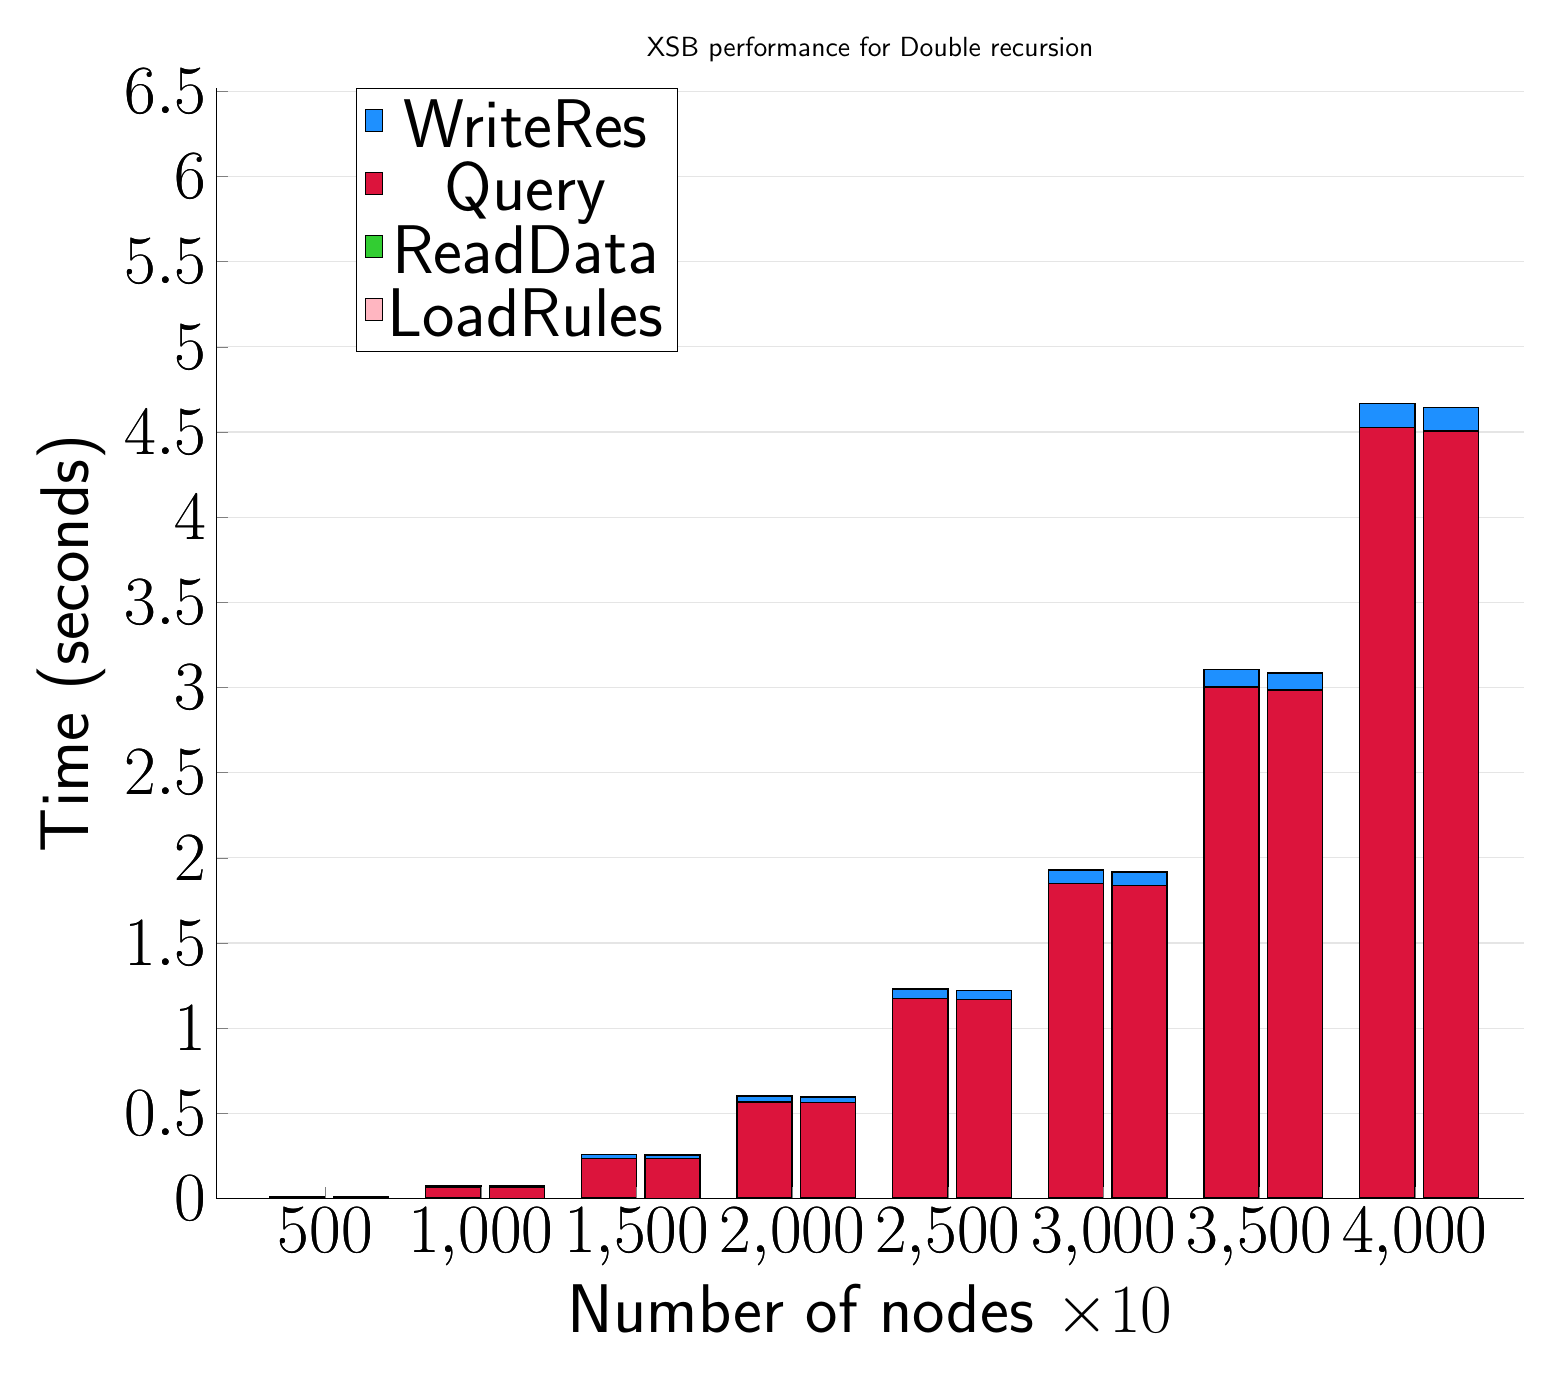
\begin{tikzpicture}
\begin{axis}[
   ybar stacked,
   title={XSB performance for Double recursion},
   bar shift=-10pt,
   width=1.5\textwidth,
   bar width=0.7cm,
   ymajorgrids, tick align=inside,
   major grid style={draw=gray!20},
   xtick=data,
   ymin=0, ymax=6.52002317905426,
   axis x line*=bottom,
   axis y line*=left,
   enlarge x limits=0.1,
   legend style={
       at={(0.23, 1)},
       anchor=north,
       legend columns=1,
       font=\Huge,
   },
   ylabel={Time (seconds)},
   xlabel={Number of nodes $\times 10$},
   label style={font=\Huge},
   tick label style={font=\Huge},
]
\addlegendimage{fill=DodgerBlue, draw=black, line width=0.2pt}
\addlegendentry{WriteRes}
\addlegendimage{fill=Crimson, draw=black, line width=0.2pt}
\addlegendentry{Query}
\addlegendimage{fill=LimeGreen, draw=black, line width=0.2pt}
\addlegendentry{ReadData}
\addlegendimage{fill=LightPink, draw=black, line width=0.2pt}
\addlegendentry{LoadRules}
\addplot +[fill=LightPink, draw=black, line width=0.5pt] coordinates {
    (500, 0.0010662078857421888)
    (1000, 0.001069474220275881)
    (1500, 0.001044011116027832)
    (2000, 0.0011091470718383812)
    (2500, 0.0010732173919677731)
    (3000, 0.0010759592056274422)
    (3500, 0.0011322736740112288)
    (4000, 0.001083302497863769)
};
\addplot +[fill=LimeGreen, draw=black, line width=0.5pt] coordinates {
    (500, 0.0008016824722290039)
    (1000, 0.001351714134216309)
    (1500, 0.001883029937744141)
    (2000, 0.002444624900817869)
    (2500, 0.003077077865600585)
    (3000, 0.0035151243209838867)
    (3500, 0.004081225395202637)
    (4000, 0.004600954055786132)
};
\addplot +[fill=Crimson, draw=black, line width=0.5pt] coordinates {
    (500, 0.007842040061950686)
    (1000, 0.06608376502990723)
    (1500, 0.2337904691696167)
    (2000, 0.5638386964797976)
    (2500, 1.1712010145187381)
    (3000, 1.844814229011536)
    (3500, 2.9986293077468877)
    (4000, 4.52002317905426)
};
\addplot +[fill=DodgerBlue, draw=black, line width=0.5pt] coordinates {
    (500, 0.002534842491149906)
    (1000, 0.009842729568481447)
    (1500, 0.023076581954956092)
    (2000, 0.03546550273895262)
    (2500, 0.054489684104918036)
    (3000, 0.07987043857574301)
    (3500, 0.101319289207458)
    (4000, 0.1411851882934579)
};
\end{axis}
\begin{axis}[
   ybar stacked,
   bar shift=13pt,
   width=1.5\textwidth,
   bar width=0.7cm,
   ymajorgrids, tick align=inside,
   major grid style={draw=none},
   xtick=data,
   ymin=0, ymax=6.52002317905426,
   axis x line*=none,
   axis y line*=none,
   enlarge x limits=0.1,
   label style={font=\Huge},
   tick label style={font=\Huge},
]
\addplot +[fill=LightPink, draw=black, line width=0.5pt] coordinates {
    (500, 0.0006204)
    (1000, 0.0006066000000000002)
    (1500, 0.0006002000000000001)
    (2000, 0.0006371000000000004)
    (2500, 0.0006150999999999997)
    (3000, 0.0006217)
    (3500, 0.0006406000000000001)
    (4000, 0.0006160000000000001)
};
\addplot +[fill=LimeGreen, draw=black, line width=0.5pt] coordinates {
    (500, 0.0005870999999999995)
    (1000, 0.0010638)
    (1500, 0.0015355)
    (2000, 0.0020614)
    (2500, 0.0026220999999999996)
    (3000, 0.0030441)
    (3500, 0.0035825999999999996)
    (4000, 0.0039934)
};
\addplot +[fill=Crimson, draw=black, line width=0.5pt] coordinates {
    (500, 0.007741)
    (1000, 0.06547050000000001)
    (1500, 0.23226030000000003)
    (2000, 0.5598783999999999)
    (2500, 1.1648720000000001)
    (3000, 1.8355333000000003)
    (3500, 2.9813151)
    (4000, 4.500052500000001)
};
\addplot +[fill=DodgerBlue, draw=black, line width=0.5pt] coordinates {
    (500, 0.0022398000000000006)
    (1000, 0.009411700000000002)
    (1500, 0.022235599999999994)
    (2000, 0.034432000000000004)
    (2500, 0.05318070000000001)
    (3000, 0.0781804)
    (3500, 0.10023200000000002)
    (4000, 0.13836970000000015)
};
\end{axis}
\end{tikzpicture}

\end{document}
